\documentclass[aspectratio=169]{beamer}
\usepackage[utf8]{inputenc}
\usepackage{hyperref}
\usepackage{amsmath,amsfonts,amsthm,bm}
\usepackage{color}
\usepackage{graphicx} % Allows including images
\usepackage{subcaption}
\usepackage{booktabs} % Allows the use of \toprule, \midrule and \bottomrule in tables
\usepackage{tikz}
\usetikzlibrary{automata,positioning,shapes.geometric,shapes.misc,arrows}
%\usepackage{pgfplots}
\usepackage{listings}
\usepackage{courier}
\usepackage[version=4]{mhchem}
\usepackage{array}

\lstset{ %
    basicstyle=\scriptsize\ttfamily, % fonts that are used for the code
    breakatwhitespace=false,         % sets if automatic breaks should only happen at whitespace
%breaklines=true,                 % sets automatic line breaking
%captionpos=b,                    % sets the caption-position to bottom
    commentstyle=\color{gray}\textit,    % comment style
    keepspaces=true,                 % keeps spaces in text, useful for keeping indentation of code (possibly needs columns=flexible)
    keywordstyle=\color{blue},       % keyword style
    language=Python,                 % the language of the code
%otherkeywords={*,...},          % if you want to add more keywords to the set
    rulecolor=\color{black},         % if not set, the frame-color may be changed on line-breaks within not-black text (e.g. comments (green here))
    showspaces=false,                % show spaces everywhere adding particular underscores; it overrides 'showstringspaces'
    showstringspaces=false,          % underline spaces within strings only
    showtabs=false,                  % show tabs within strings adding particular underscores
    stringstyle=\color{red}, % string literal style
    tabsize=4,                       % sets default tabsize to 2 spaces
    columns=fixed                    % Using fixed column width (for e.g. nice alignment)
}

\hypersetup{
    colorlinks=true,
    linkcolor=red,
    filecolor=magenta,
    urlcolor=red,
}

\DeclareMathOperator*{\argmax}{argmax}
\DeclareMathOperator*{\argmin}{argmin}
\let \vec \mathbf

\newcommand{\classname}{NANO266}
\newcommand{\classyear}{Fall 2024}
\mode<presentation> {
    \usetheme{CambridgeUS}
    \setbeamertemplate{footline}[text line]{%
        \parbox{\linewidth}{\vspace*{-8pt}\classname\hfill\classyear\hfill\insertpagenumber}}

    %\setbeamertemplate{footline}[page number]
    \setbeamertemplate{navigation symbols}{}
}


\title[\classname Transition States]{\classname~- Quantum Mechanical Modeling of Materials and Nanostructures\\Transition States}

\author{Shyue Ping Ong}
\institute[UCSD]{University of California, San Diego\\
\medskip
}
\date{\classyear} % Date, can be changed to a custom date

\begin{document}


    \begin{frame}
        \titlepage % Print the title page as the first slide
    \end{frame}


    \begin{frame}{Transition states}
Particular configuration along a reaction coordinate corresponding to the highest potential energy along the reaction coordinate.
\begin{figure}
    \centering
    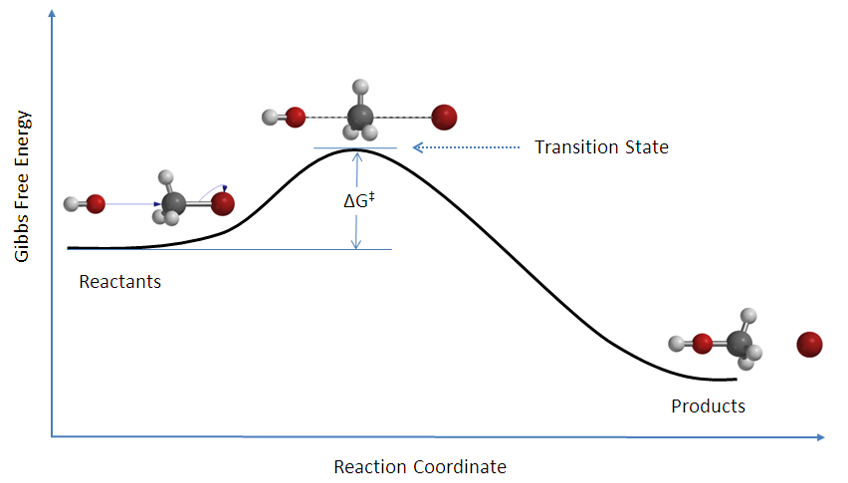
\includegraphics[width=0.5\linewidth]{lectures/figures/12_transition_state.png}
    \caption{\ce{HO- + CH3Br \rightarrow [HO---CH3---Br]^\ddag \rightarrow CH3OH + Br}}
\end{figure} 

    \end{frame}

\begin{frame}{Applications}
Reactions
\begin{itemize}
    \item Activated states
    \item Barriers to reactions
    \item Lowest energy pathway from reactant to products
    \item Rates of reactions
\end{itemize}

Diffusion
\begin{itemize}
    \item Activation energies for migration
    \item E.g., migration of defects (radiation damage), Li migration for batteries
\end{itemize}
\end{frame} 

\begin{frame}{Potential Energy Surface}
\begin{figure}
    \centering
    \begin{subfigure}{0.45\textwidth}
        \centering
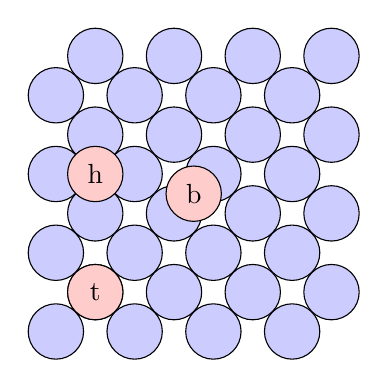
\begin{tikzpicture}[
scale=0.5,
atom/.style={circle,draw=black,fill=white!80!blue,minimum size=20},
dopant/.style={circle,draw=black,fill=white!80!red,minimum size=20}
]
\foreach \i in {1,...,4}
{
    \foreach \j in {1,...,4}
    {
        \pgfmathtruncatemacro{\label}{\i\j};
        \node[atom] (\label) at (2*\i,2*\j) { };
        \node[atom] (\label) at (2*\i+1,2*\j+1) { };
    }
}
\node[dopant] () at (3,3) {t};
\node[dopant] () at (3,6) {h};
\node[dopant] () at (5.5,5.5) {b};
\end{tikzpicture}
\caption{Symmetrically distinct sites on a fcc (100) surface, e.g., Au on Cu(100). h: hollow, b: bridge, t: top.}
    \end{subfigure}
    \begin{subfigure}{0.45\textwidth}
        \centering
        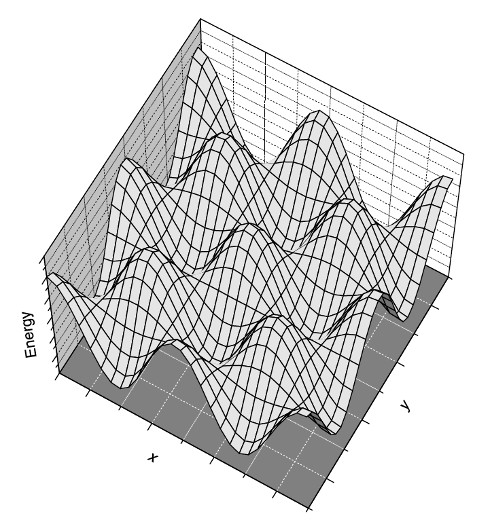
\includegraphics[width=0.8\linewidth]{lectures/figures/12_PES.png}
    \caption{Potential energy surface $E(x,y)$.}
    \end{subfigure}
\end{figure} 
\end{frame} 

\begin{frame}{Rate Equation}

\begin{equation*}
r = \nu e^{-\frac{E_a}{k_bT}}
\end{equation*} 

\begin{itemize}
    \item $\nu$: Attempt frequency. Atomic vibrations are on the order of 0.1-1ps, which implies $\nu \approx 10^{12}-10^{13}$. This is a frequently used approximation to avoid having to undertake a potentially complex calculation of the frequency directly.
    \item $k_b$: Boltzmann's constant.
    \item $T$: Temperature.
    \item $E_a$: Activation energy. $\approx 60$ meV change in $E_a$ leads to an order of magnitude change in the rate at room temperature (300K).
\end{itemize}

\end{frame} 
\begin{frame}{Nudged Elastic Band (NEB) Method}
\begin{columns}
\column{0.5\textwidth}
Method for finding the minimum energy path (MEP) when initial and final endpoints are known.\newline
\newline 
Initial guesses for MEP typically given by linear interpolations between the start ($\{\vec{r_i}\}$) and end points ($\{\vec{r_f}\}$). The interpolated points are known as images.

\begin{equation*}
\{\vec{r_x}\} = x \{\vec{r_i}\} + (1-x)\{\vec{r_f}\}
\end{equation*} 
\column{0.5\textwidth}
\begin{figure}
    \centering
    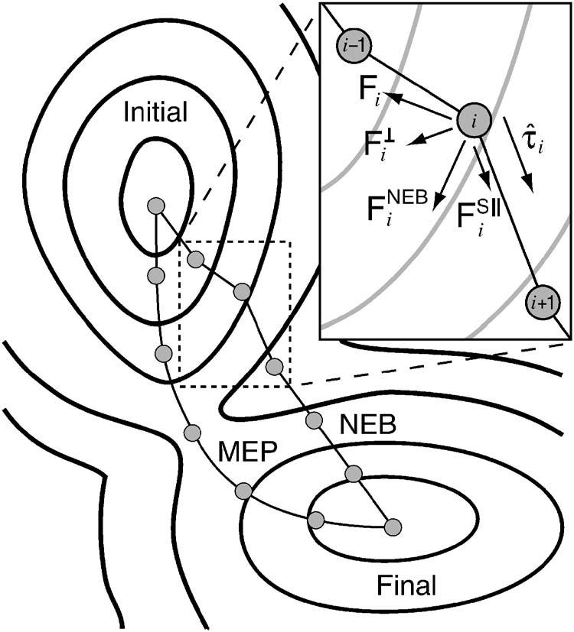
\includegraphics[width=0.55\linewidth]{lectures/figures/12_NEB.png}
    \caption{Conceptually similar to adding springs between images. Images are moved in accordance to the forces.\cite{henkelmanClimbingImageNudged2000}}
\end{figure} 
\end{columns} 
\end{frame} 


\begin{frame}{Climbing Image NEB}
\begin{columns}
\column{0.5\textwidth}

\begin{figure}
    \centering
    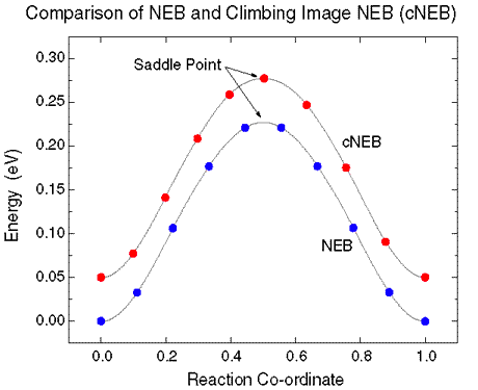
\includegraphics[width=\linewidth]{lectures/figures/12-CINEB.png}
    \caption{CI NEB vs vanilla NEB}
\end{figure} 

\column{0.5\textwidth}
\begin{itemize}
    \item Modification of NEB forces to move the potential energy surface along the elastic band and down the potential surface perpendicular to the band.\cite{henkelmanClimbingImageNudged2000} 
    \item Other images in the band define the one degree of freedom for which a maximization of the energy is carried out.
    \item Good approximation of saddle point. 
    \item No additional cost.
\end{itemize}
\end{columns} 
\end{frame} 

\begin{frame}{CI vs regular NEB}
\begin{figure}
    \centering
    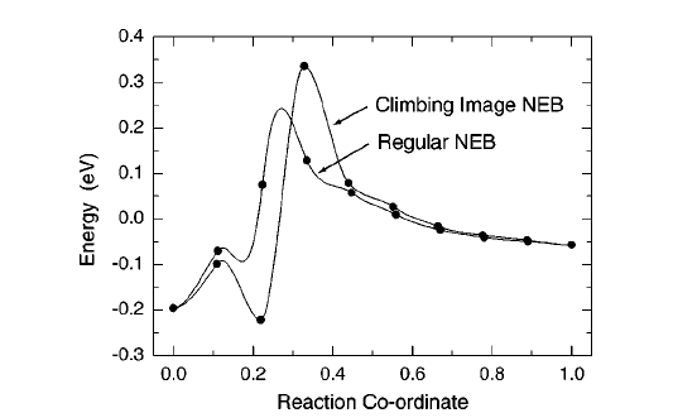
\includegraphics[width=0.6\linewidth]{lectures/figures/12-CINEB_2.png}
    \caption{MEP of \ce{CH4} dissociative adsorption on Ir(111) surface.\cite{henkelmanClimbingImageNudged2000}}
\end{figure} 
\end{frame} 

\begin{frame}{Variable Springs}

\begin{figure}
    \centering
    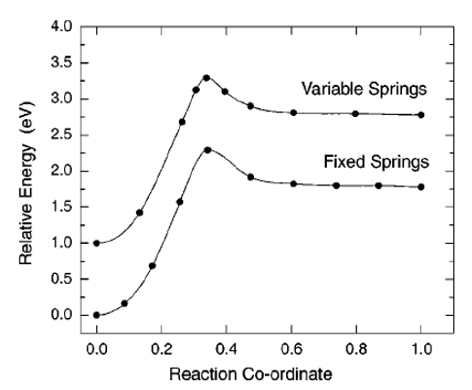
\includegraphics[width=0.4\linewidth]{lectures/figures/12-variable_springs.png}
    \caption{MEP for \ce{H2} dissociative adsorption on Si(100) surface. Spring strength is increased near saddle point to increase resolution.\cite{henkelmanClimbingImageNudged2000}}
\end{figure} 
\end{frame} 

\begin{frame}{NEB calculation procedure}
\begin{figure}
    \centering
    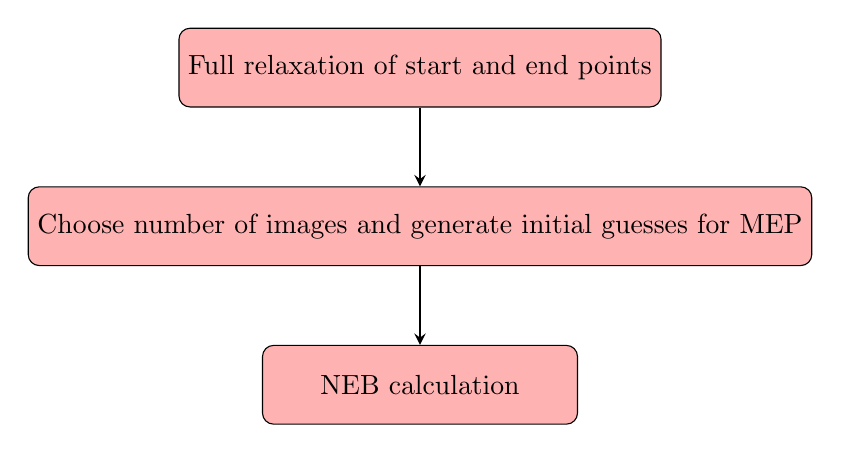
\begin{tikzpicture}[node distance=1cm]
        \tikzstyle{roundrect} = [rectangle, rounded corners, minimum width=4cm, minimum height=1cm,text centered, draw=black, fill=red!30]
        \tikzstyle{arrow} = [thick,->,>=stealth]
        \node (node1) [roundrect] {Full relaxation of start and end points};
        \node (node2) [roundrect, below=of node1] {Choose number of images and generate initial guesses for MEP};
        \node (node3) [roundrect, below=of node2] {NEB calculation};

        \draw [arrow] (node1) -- (node2);
        \draw [arrow] (node2) -- (node3);
    \end{tikzpicture}
\end{figure} 
\end{frame} 

\begin{frame}{Challenges in NEB calculations}
\begin{enumerate}
    \item Stability of calculation depends on number of images. Too few images $\implies$ lack of resolution. Too many $\implies$ unstable convergence.
    \item Linear interpolation between start and end points may lead to very bad guesses for MEP. 
    \item Convergence towards MEP may be extremely slow.
    \item Force convergence criteria typically much more stringent.
    \item Guess for the MEP may bias the final solution.
\end{enumerate}
\end{frame} 

\begin{frame}{Example: Oxygen vacancy diffusion in YSZ}
\begin{figure}
    \centering
    \begin{subfigure}{0.45\textwidth}
        \centering
        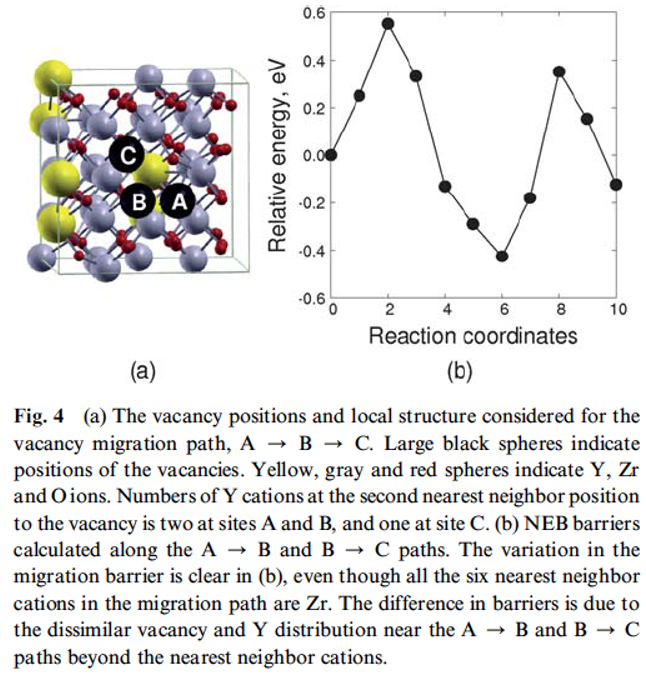
\includegraphics[width=0.8\linewidth]{lectures/figures/12-O_diffusion_in_YSZ_1.png}
    \end{subfigure}
    \begin{subfigure}{0.45\textwidth}
        \centering
        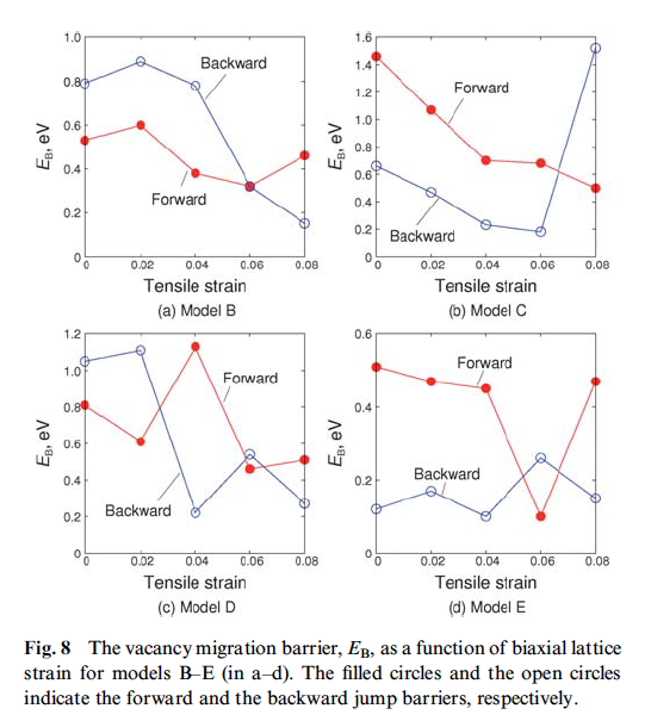
\includegraphics[width=0.8\linewidth]{lectures/figures/12-O_diffusion_in_YSZ_2.png}
    \end{subfigure}
    \caption{\cite{kushimaOxygenIonDiffusivity2010}}
\end{figure} 
\end{frame} 

\begin{frame}{Example: Hydrogen diffusion on TM surfaces}
\begin{figure}
    \centering
    \begin{subfigure}{0.45\textwidth}
        \centering
        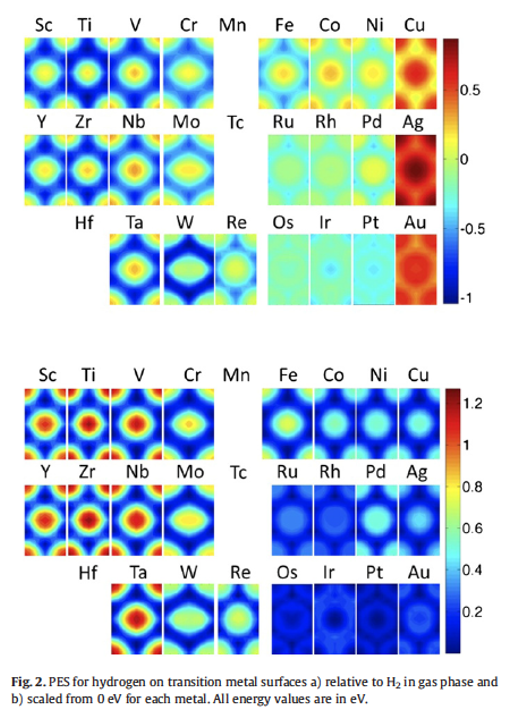
\includegraphics[width=0.65\linewidth]{lectures/figures/12-H_TM_1.png}
    \end{subfigure}
    \begin{subfigure}{0.45\textwidth}
        \centering
        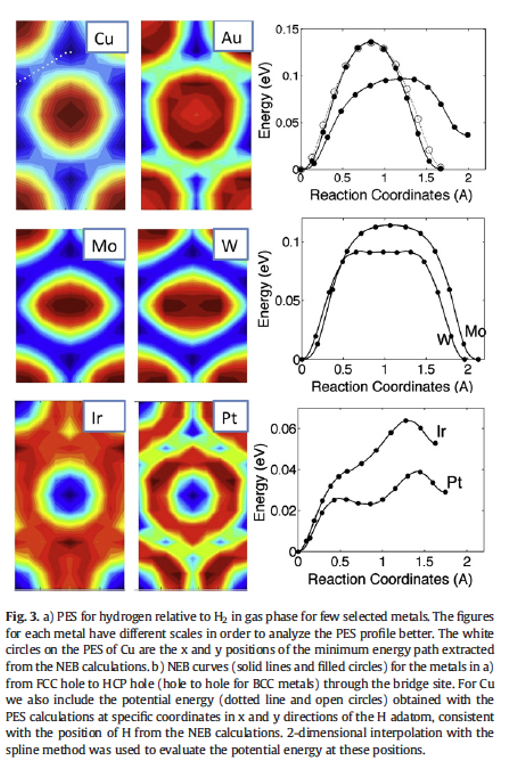
\includegraphics[width=0.6\linewidth]{lectures/figures/12-H_TM_2.png}
    \end{subfigure}
    \caption{\cite{kristinsdottirSystematicDFTStudy2012}}
\end{figure} 
\end{frame} 

\begin{frame}{Example: Methanol oxidation on Cu surfaces}
\begin{figure}
    \centering
    \begin{subfigure}{0.45\textwidth}
        \centering
        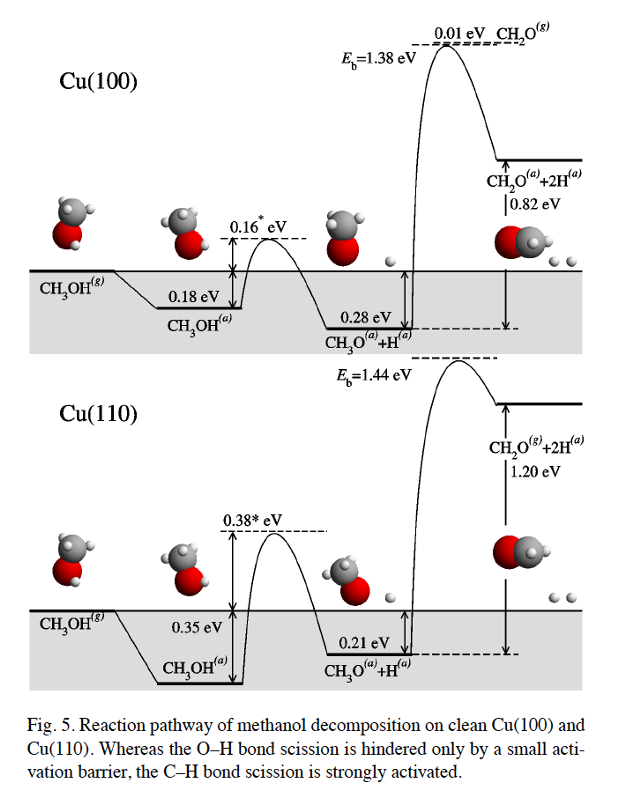
\includegraphics[width=0.65\linewidth]{lectures/figures/12-Methanol_Cu_1.png}
    \end{subfigure}
    \begin{subfigure}{0.45\textwidth}
        \centering
        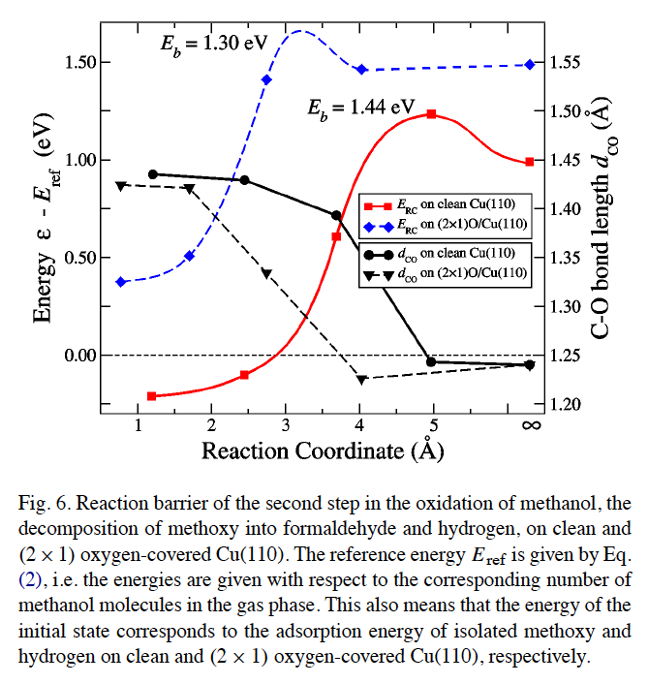
\includegraphics[width=0.8\linewidth]{lectures/figures/12-Methanol_Cu_2.png}
    \end{subfigure}
    \caption{\cite{sakongDensityFunctionalTheory2005}}
\end{figure} 
\end{frame} 


\begin{frame}{Example: Spinel cathodes for multivalent batteries}
\begin{figure}
    \centering
    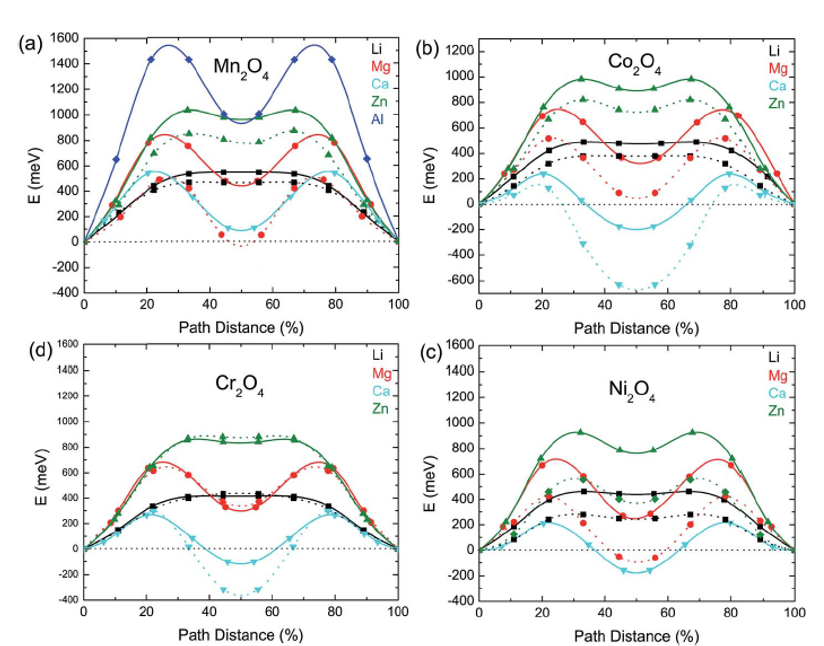
\includegraphics[width=0.5\linewidth]{lectures/figures/12-Multivalent_Cathodes.png}
    \caption{MEP for migration of ions in spinel \ce{B2O4}.\cite{liuSpinelCompoundsMultivalent2014}}
\end{figure} 
\end{frame} 

\begin{frame}{Kinetic Monte Carlo}
MC simulation method for the time evolution of natural processes. For studies of diffusivity or reaction rates, requires as input environment-dependent activation barriers (usually from NEB).

Basic algorithm:
\begin{enumerate}
    \item Start with an equilibrium atomic arrangement.
    \item Determine  migration probabilities $\Gamma$ based on the paths available. $\Gamma$ is calculated based on Arrhenius form.
    \item Sample a random number in $(0,1]$, and the migration event $k$ is chosen such that:
    \begin{equation*}
    \frac{1}{\Gamma_{tot}} \sum_{m=1}^{k-1} \Gamma_m < \rho \leq \frac{1}{\Gamma_{tot}} \sum_{m=1}^{k} \Gamma_m 
    \end{equation*} 
    \item Time is updated by $\Delta t = - \frac{1}{\Gamma_{tot}} \log \eta$ where $\eta \in (0,1]$

\end{enumerate}

\end{frame} 

\begin{frame}{Example: Diffusion in \ce{LiCoO2}}
\begin{figure}
    \centering
    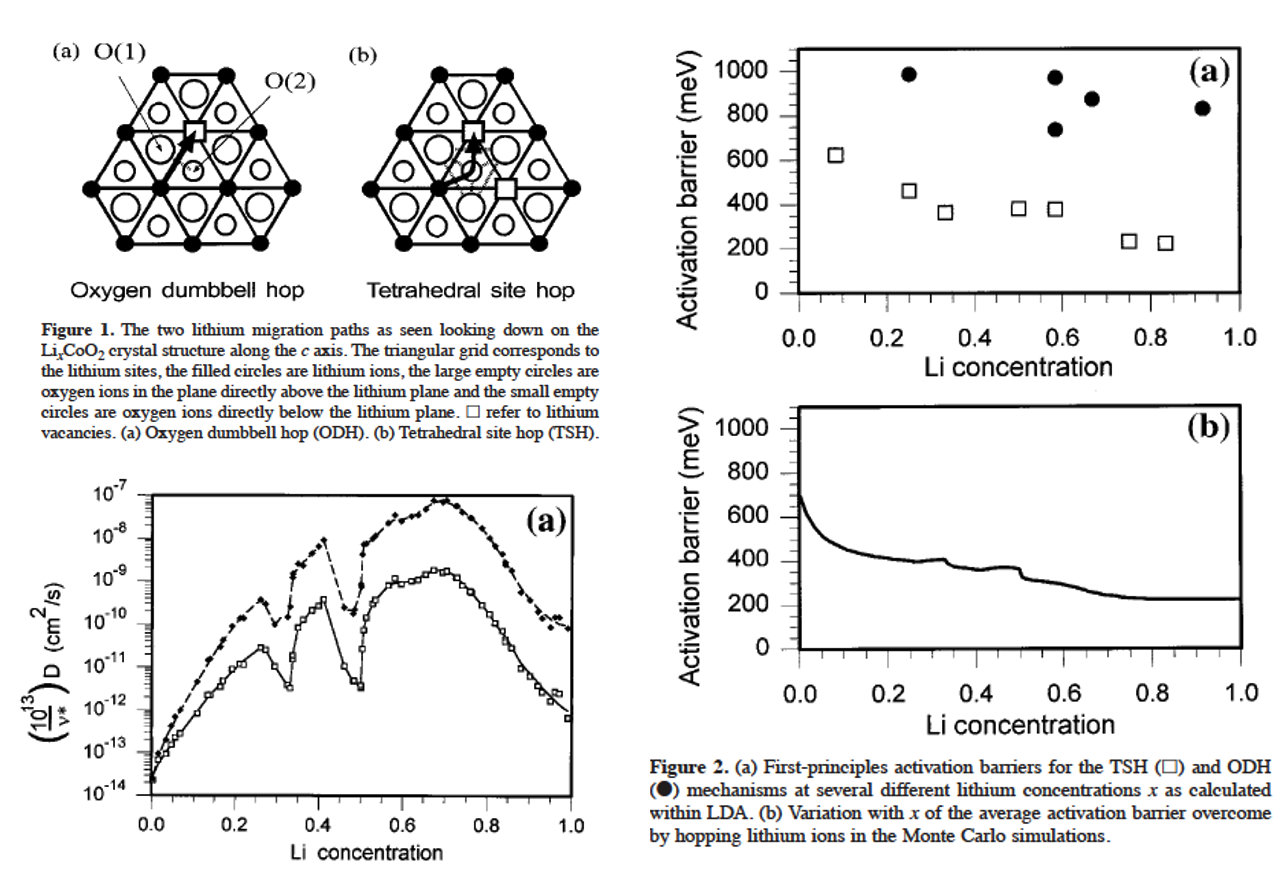
\includegraphics[width=0.6\linewidth]{lectures/figures/12-LCO_Diffusion.png}
    \caption{Lithium Diffusion in Layered \ce{Li_xCoO2}\cite{vandervenLithiumDiffusionLayered2000}}
\end{figure} 
\end{frame} 


\begin{frame}{NEB+Percolation Theory}
\begin{figure}
    \centering
    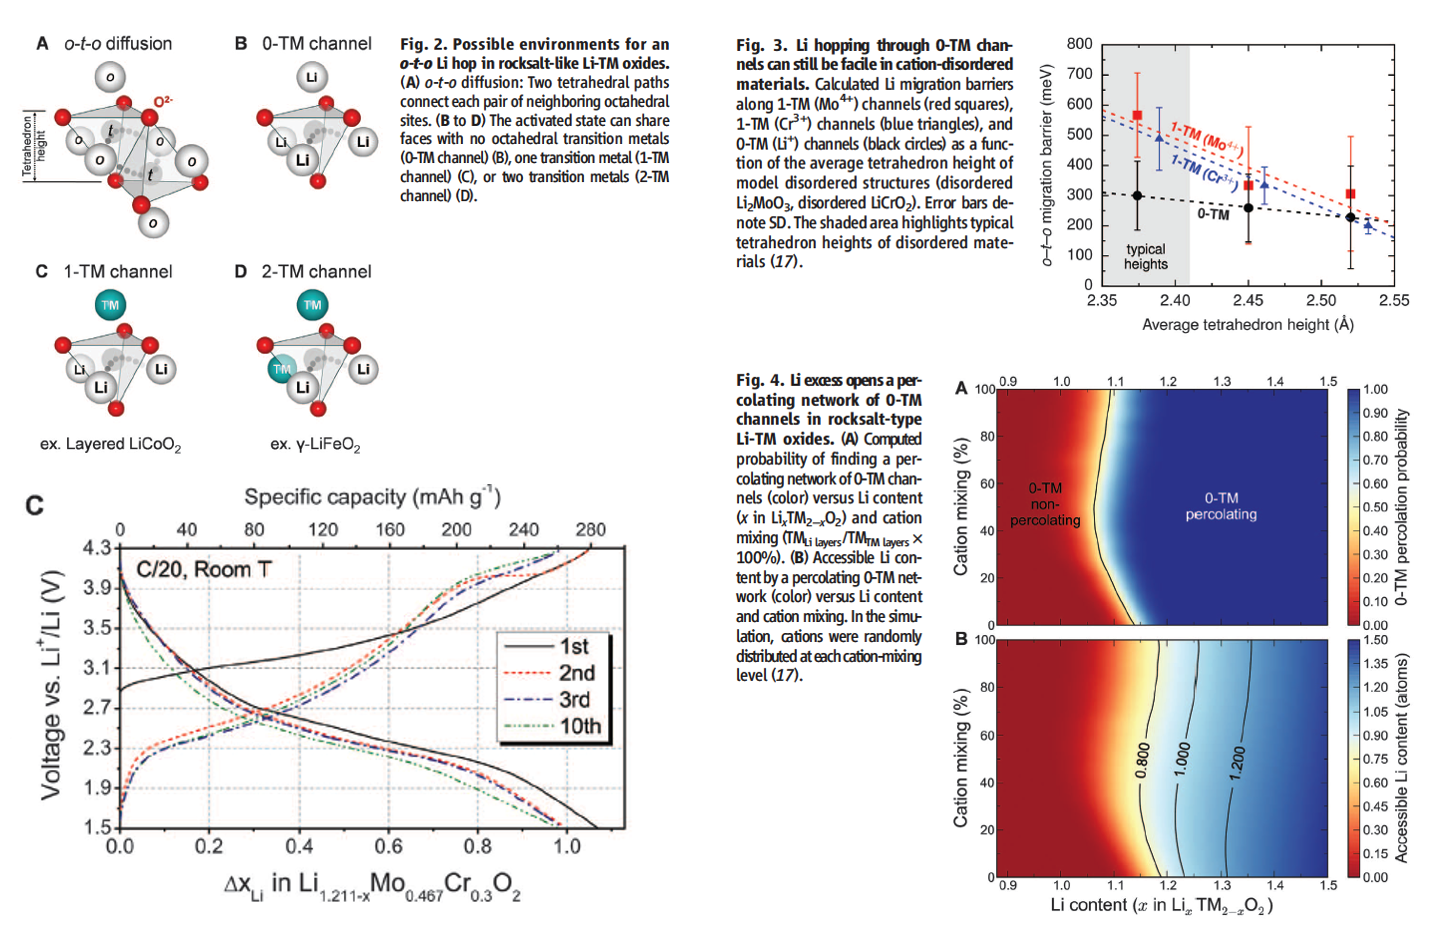
\includegraphics[width=0.6\linewidth]{lectures/figures/12-Percolation.png}
    \caption{Unlocking the potential of cation-disordered oxides for rechargeable lithium batteries.\cite{leeUnlockingPotentialCationdisordered2014}}
\end{figure} 
\end{frame} 

\begin{frame}{Growing String Method}
\begin{columns}
\column{0.5\textwidth}

\begin{figure}
    \centering
    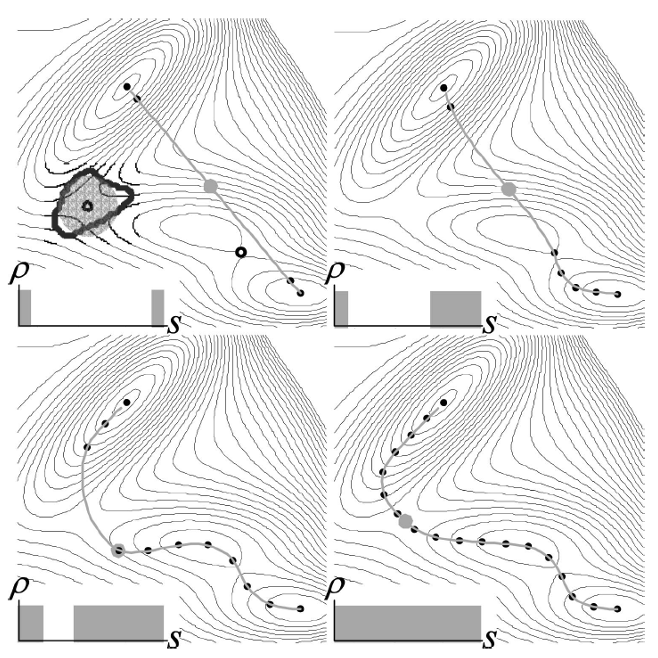
\includegraphics[width=0.8\linewidth]{lectures/figures/12-Growing_String.png}
    \caption{Growing string on Muller Brown PES.\cite{petersGrowingStringMethod2004}}
\end{figure} 

\column{0.5\textwidth}

\begin{itemize}
    \item Begins as two string fragments, one associated with the reactants and the other with the products. 
    \item Each string fragment is grown separately until the fragments converge.
    \item Once the two fragments join, the full string moves toward the MEP.
    \item Typically finds saddle points much more quickly when linearly interpolated guess is very far from MEP.
\end{itemize}

\end{columns} 
\end{frame} 


    \begin{frame}[allowframebreaks]{Bibliography}
        \bibliographystyle{unsrt}
        \bibliography{refs}
    \end{frame}



    \begin{frame}
        \Huge{\centerline{The End}}
    \end{frame}

\end{document}

